% fig_residual_comparison.tex
% Stacked comparison: charging residual floor and I_fund threshold by method
% Left axis: residual RMS [pu]; Right axis (implied): threshold [pu]
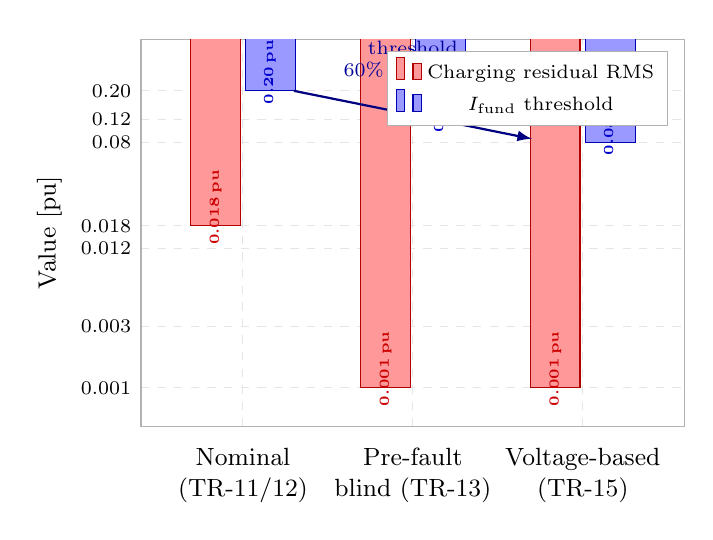
\begin{tikzpicture}
\begin{axis}[
  name            = residax,
  ybar,
  bar width       = 18pt,
  width           = 0.70\textwidth,
  height          = 6.5cm,
  enlarge x limits= 0.30,
  ylabel          = {Value [pu]},
  ylabel style    = {font=\small},
  ymode           = log,
  ymin            = 5e-4,
  ymax            = 0.5,
  ytick           = {0.001, 0.003, 0.012, 0.018, 0.08, 0.12, 0.20},
  yticklabels     = {0.001, 0.003, 0.012, 0.018, 0.08, 0.12, 0.20},
  yticklabel style= {font=\scriptsize},
  xtick           = {1, 2, 3},
  xticklabels     = {
    {Nominal\\(TR-11/12)},
    {Pre-fault\\blind (TR-13)},
    {Voltage-based\\(TR-15)}
  },
  xticklabel style= {font=\small, align=center},
  legend style    = {at={(0.97,0.97)}, anchor=north east,
                     font=\scriptsize, draw=gray!60},
  legend columns  = 1,
  grid            = major,
  grid style      = {gray!20, dashed},
  tick style      = {draw=none},
  axis line style = {gray!60},
]

% Residual RMS bars (red)
\addplot[fill=red!40, draw=red!70!black]
  coordinates {(1,0.018) (2,0.001) (3,0.001)};
\addlegendentry{Charging residual RMS}

% I_fund threshold bars (blue, offset)
\addplot[fill=blue!40, draw=blue!70!black]
  coordinates {(1,0.200) (2,0.120) (3,0.080)};
\addlegendentry{$I_{\rm fund}$ threshold}

% ---- Value annotations ----------------------------------------------------
% Residual
\node[font=\tiny\bfseries, red!80!black, rotate=90]
  at (axis cs:0.84, 0.025) {0.018\,pu};
\node[font=\tiny\bfseries, red!80!black, rotate=90]
  at (axis cs:1.84, 0.0014) {0.001\,pu};
\node[font=\tiny\bfseries, red!80!black, rotate=90]
  at (axis cs:2.84, 0.0014) {0.001\,pu};

% Threshold
\node[font=\tiny\bfseries, blue!80!black, rotate=90]
  at (axis cs:1.16, 0.28) {0.20\,pu};
\node[font=\tiny\bfseries, blue!80!black, rotate=90]
  at (axis cs:2.16, 0.168) {0.12\,pu};
\node[font=\tiny\bfseries, blue!80!black, rotate=90]
  at (axis cs:3.16, 0.112) {0.08\,pu};

% ---- Reduction annotation --------------------------------------------------
\node[font=\scriptsize, blue!60!black, align=center]
  at (axis cs:2.0, 0.35) {threshold\\60\% reduction};
\draw[-latex, blue!50!black, thick]
  (axis cs:1.3, 0.20) -- (axis cs:2.7, 0.085);

\end{axis}
\end{tikzpicture}
